
Este capítulo reúne os modelos elaborados para a plataforma. A Seção~\ref{sec:casos-de-uso} apresenta o diagrama de casos de uso, a Seção~\ref{sec:arquitetura-plataforma} descreve a arquitetura em camadas e a Seção~\ref{sec:modelo-dados} apresenta o modelo do banco de dados.

\section{Diagrama de Casos de Uso}
\label{sec:casos-de-uso}

Um diagrama de casos de uso mostra um conjunto de casos de uso, os atores e os relacionamentos entre eles. Na UML, esse diagrama é usado para organizar e modelar o comportamento de um sistema tal como ele é percebido de fora, isto é, o que o sistema oferece a quem o utiliza, sem descrever como cada funcionalidade é implementada \cite{booch2006uml}. Cada caso de uso representa uma tarefa que envolve interação com o sistema, e os atores podem ser pessoas ou outros sistemas \cite{sommerville2018}. Neste trabalho, o diagrama serviu para delimitar os fluxos da plataforma e para derivar os requisitos apresentados no Capítulo~\ref{cap:proposta}.

A Figura~\ref{fig:casos-de-uso} apresenta o diagrama da plataforma, com todos os casos de uso e quatro atores. O Visitante usa a plataforma sem conta: pode cadastrar-se, autenticar-se, usar a IDE e criar linguagens personalizadas, mas a linguagem criada fica apenas no armazenamento local do navegador. O Usuário autenticado tem os mesmos recursos da IDE e acrescenta o gerenciamento do perfil, a gravação das linguagens no servidor e o compartilhamento e a importação de linguagens da comunidade. O Aluno e o Professor são especializações do Usuário autenticado: herdam os casos de uso dele e acrescentam, respectivamente, a participação em turmas, com consulta e submissão de exercícios, e a gestão pedagógica de turmas, exercícios e listas.

Os atores correspondem aos papéis gravados no banco de dados (Seção~\ref{sec:modelo-dados}) da seguinte forma. O papel \texttt{STUDENT} corresponde ao Aluno. Os papéis \texttt{TEACHER} e \texttt{ADMIN} correspondem ao Professor, porque a interface oferece ao administrador os mesmos recursos pedagógicos do professor. O papel \texttt{COMMUNITY} corresponde ao Usuário autenticado que não participa de turmas. O papel \texttt{SYSTEM} é interno, não representa uma pessoa usando a plataforma e por isso não aparece no diagrama.

\begin{figure}[htbp]
\centering
\caption{Diagrama de casos de uso da plataforma.}
\label{fig:casos-de-uso}
\resizebox{\linewidth}{!}{%
\begin{tikzpicture}[x=1cm,y=1cm,uc/.append style={font=\footnotesize,minimum width=3.6cm,minimum height=.9cm}]
% Fronteira do sistema.
\draw[thick] (2.9,1.3) rectangle (18.3,-11.8);
\node[font=\small\bfseries] at (10.6,.85) {Plataforma educacional web};
% Lado esquerdo: casos de uso do Visitante e do Usuário autenticado, em duas
% colunas intercaladas, para que as ligações passem entre as elipses.
\node[uc] (ucCad)  at (5.0,0.0)   {Cadastrar-se};
\node[uc] (ucAut)  at (8.4,-1.1)  {Autenticar-se};
\node[uc] (ucLing) at (5.0,-2.2)  {Criar e gerenciar\\linguagens personalizadas};
\node[uc] (ucAtiv) at (8.4,-3.3)  {Ativar linguagem\\no editor};
\node[uc] (ucEdit) at (5.0,-4.4)  {Editar código na IDE};
\node[uc] (ucArq)  at (8.4,-5.5)  {Gerenciar arquivos\\do projeto};
\node[uc] (ucExec) at (5.0,-6.6)  {Executar programa\\no terminal};
\node[uc] (ucTok)  at (8.4,-7.7)  {Inspecionar \textit{tokens} e\\código intermediário};
\node[uc] (ucDep)  at (5.0,-8.8)  {Depurar execução\\passo a passo};
\node[uc] (ucPer)  at (8.4,-9.9)  {Gerenciar perfil};
\node[uc] (ucCom)  at (5.0,-11.0) {Compartilhar e importar\\linguagens da comunidade};
% Lado direito: casos de uso do Aluno (acima) e do Professor (abaixo).
\node[uc] (ucIng)  at (16.2,0.0)   {Ingressar em turma};
\node[uc] (ucCons) at (12.8,-1.1)  {Consultar listas\\e exercícios};
\node[uc] (ucSub)  at (16.2,-2.2)  {Submeter solução\\de exercício};
\node[uc] (ucVer)  at (12.8,-3.3)  {Consultar veredito\\e histórico};
\node[uc] (ucTur)  at (16.2,-4.4)  {Gerenciar turmas};
\node[uc] (ucMem)  at (12.8,-5.5)  {Gerenciar membros\\da turma};
\node[uc] (ucEx)   at (16.2,-6.6)  {Gerenciar exercícios\\e casos de teste};
\node[uc] (ucVinc) at (12.8,-7.7)  {Vincular linguagem\\a exercício ou lista};
\node[uc] (ucLis)  at (16.2,-8.8)  {Gerenciar listas\\de exercícios};
\node[uc] (ucPub)  at (12.8,-9.9)  {Publicar lista\\para a turma};
\node[uc] (ucAva)  at (16.2,-11.0) {Acompanhar e avaliar\\submissões};
% Atores.
\pic at (0.8,-1.6) {ator}; \node[font=\small] at (0.8,-3.25) {Visitante};
\pic at (0.8,-7.9) {ator}; \node[font=\small,align=center] at (0.8,-9.85) {Usuário\\autenticado};
\pic at (21.0,-0.6) {ator}; \node[font=\small] at (21.0,-2.25) {Aluno};
\pic at (19.9,-6.9) {ator}; \node[font=\small] at (19.9,-8.55) {Professor};
% Nota (comentário UML), ligada ao ator Visitante por linha tracejada.
\node[font=\footnotesize,text width=5.4cm,align=left,inner sep=5pt] (nota) at (2.6,2.75)
  {O acesso pelo ator Visitante não exige \textit{login}. Para os demais atores, todas as operações exigem \textit{login}.};
\draw (nota.south west) -- (nota.south east) -- ([yshift=-7pt]nota.north east)
      -- ([xshift=-7pt]nota.north east) -- (nota.north west) -- cycle;
\draw ([xshift=-7pt]nota.north east) -- ([xshift=-7pt,yshift=-7pt]nota.north east) -- ([yshift=-7pt]nota.north east);
\coordinate (vx) at (0.8,0);
\draw[dashed] (nota.south -| vx) -- (0.8,-1.38);
% Generalização: Aluno e Professor herdam do Usuário autenticado.
\draw[heranca] (21.0,-2.65) -- (21.0,-12.6) -- (0.8,-12.6) -- (0.8,-10.55);
\draw[heranca] (19.9,-8.95) -- (19.9,-12.6) -- (0.8,-12.6) -- (0.8,-10.55);
% Associações: partem de alturas ligeiramente diferentes junto a cada ator.
\begin{scope}[on background layer]
\foreach \d/\o in {ucCad/0.8,ucAut/0.6,ucLing/0.4,ucAtiv/0.2,ucEdit/0,ucArq/-0.2,ucExec/-0.4,ucTok/-0.6,ucDep/-0.8}
  \draw[liga] (1.15,{-2.0+\o}) -- (\d);
\foreach \d/\o in {ucLing/0.8,ucAtiv/0.6,ucEdit/0.4,ucArq/0.2,ucExec/0,ucTok/-0.2,ucDep/-0.4,ucPer/-0.6,ucCom/-0.8}
  \draw[liga] (1.15,{-8.3+\o}) -- (\d);
\foreach \d/\o in {ucIng/0.45,ucCons/0.15,ucSub/-0.15,ucVer/-0.45}
  \draw[liga] (20.65,{-1.0+\o}) -- (\d);
\foreach \d/\o in {ucTur/0.75,ucMem/0.5,ucEx/0.25,ucVinc/0,ucLis/-0.25,ucPub/-0.5,ucAva/-0.75}
  \draw[liga] (19.55,{-7.3+\o}) -- (\d);
\end{scope}
\end{tikzpicture}}
\legend{Fonte: elaborado pelo autor.}
\end{figure}
\FloatBarrier

\section{Modelagem da Arquitetura da Plataforma}
\label{sec:arquitetura-plataforma}

A organização da plataforma foi concebida sob a ótica da Separação de Responsabilidades defendida por \citeonline{martin_clean}, dividindo o projeto em três responsabilidades principais: o pacote \texttt{compiler}, responsável pelo núcleo do interpretador; o pacote \texttt{ide}, responsável pela camada de apresentação e por toda a interação com o usuário; e o serviço de \textit{back-end}, responsável pela persistência das entidades de domínio do Ambiente Virtual de Aprendizagem. Os pacotes \texttt{compiler} e \texttt{ide} são versionados em um único repositório no formato \textit{monorepo}, viabilizando o consumo direto do compilador como dependência local da IDE, sem qualquer empacotamento intermediário e sem comunicação remota entre as duas camadas. Esse consumo elimina a requisição remota na análise interativa e permite compartilhar a implementação entre navegador e servidor.

O \textit{front-end} foi implementado com o \textit{framework} Next.js, em sua arquitetura de \textit{Pages Router} e sobre o \textit{Node.js Runtime} padrão, e sobre a biblioteca React 19, utilizando TypeScript em todo o código-fonte para verificar tipos durante o desenvolvimento. As rotas de validação de submissões usam o \textit{Node.js Runtime} porque precisam de acesso pleno às APIs do Node.js. A estilização foi conduzida com Tailwind CSS em sua quarta versão, complementada por componentes das bibliotecas \textit{shadcn/ui} e \textit{Radix UI}, que fornecem primitivas de semântica e interação, sem garantir a acessibilidade da composição final \cite{radixaccess2026}. O gerenciamento de estado assíncrono foi delegado à biblioteca \textit{TanStack React Query}, responsável pela orquestração de cache, sincronização e revalidação dos dados consumidos das rotas HTTP, enquanto a validação de formulários foi modelada com a biblioteca \textit{Zod}, integrada ao \textit{React Hook Form}.

A camada de \textit{back-end} foi implementada em Python sobre o \textit{framework} FastAPI, escolhido pelas características de alto desempenho, validação automática via \textit{Pydantic} e geração automatizada de documentação OpenAPI discutidas por \citeonline{fastapi2026}. A persistência foi sustentada pelo ORM SQLAlchemy assíncrono, com versionamento de \textit{schema} via Alembic, isolando o modelo de dados das regras de negócio em conformidade com os princípios de Arquitetura Limpa apresentados por \citeonline{martin_clean}. Essa separação mantém o modelo de persistência confinado a uma camada própria, de modo que o núcleo de compilação e a interface web não dependam diretamente do banco de dados nem de suas particularidades. Não se trata de minimizar a importância da persistência, mas de restringir seu alcance: mudanças no esquema ou no mecanismo de armazenamento não devem propagar-se para as regras de tradução nem para a camada de apresentação.

O fluxo geral da Figura~\ref{fig:arquitetura-plataforma} distingue dois ambientes de execução. No navegador, os \textit{hooks} \texttt{useLexerAnalyse} e \texttt{useIntermediatorCode} e o terminal instanciam o núcleo diretamente para analisar, traduzir e executar o programa do editor. No servidor Node.js do Next.js, a rota \texttt{/api/submissions/validate} reutiliza as mesmas classes para avaliar soluções de exercícios. O serviço FastAPI fornece autenticação e recursos persistentes. Após o carregamento da aplicação, os recursos locais não exigem uma chamada a esse serviço para cada análise; isso não equivale a garantir o carregamento inicial da plataforma sem conexão.

\begin{figure}[htbp]
    \centering
    \caption[Arquitetura da plataforma.]{Arquitetura da plataforma: camadas, módulos internos e fluxos de comunicação.}
    \label{fig:arquitetura-plataforma}
    \resizebox{\linewidth}{!}{% Fonte: hooks da IDE, terminal/body.tsx e pages/api/submissions/validate.ts.
\begin{tikzpicture}[
  box/.style={draw, rounded corners, align=center, text width=11.7cm, inner sep=8pt, font=\small},
  flow/.style={-{Latex},thick},
  note/.style={font=\footnotesize,align=center,fill=white,inner sep=3pt}
]
\node[box,fill=gray!8] (browser) at (0,0) {
  \textbf{Navegador: IDE e núcleo TypeScript}\\[4pt]
  Editor + configuração da linguagem\\
  $\downarrow$\\
  \texttt{Lexer} $\rightarrow$ \textit{tokens} $\rightarrow$ \texttt{TokenIterator} + \texttt{Emitter}\\
  $\downarrow$\\
  Instruções de três endereços $\rightarrow$ \texttt{Interpreter}\\
  $\updownarrow$\\
  Terminal e depuração: entrada, saída e estado da execução
};
\node[box,fill=gray!8] (next) at (0,-5.8) {
  \textbf{Servidor Next.js: avaliação de exercícios}\\[4pt]
  \texttt{POST /api/submissions/validate}\\
  Reutiliza \texttt{Lexer}, \texttt{TokenIterator} e \texttt{Interpreter}\\
  Traduz o programa e executa os casos de teste com entrada simulada
};
\node[box,fill=gray!8] (api) at (0,-9.4) {
  \textbf{Serviço FastAPI + SQLAlchemy}\\[4pt]
  Autenticação; usuários; organizações; linguagens; turmas;\\
  exercícios; listas; submissões
};
\node[box,text width=6cm,fill=gray!8] (db) at (0,-12.1) {
  \textbf{PostgreSQL}\\Persistência das onze tabelas de domínio
};
\draw[flow] (browser.south) -- node[note] {HTTP: código, configuração e identificação do exercício\\Resposta: vereditos dos casos de teste} (next.north);
\draw[flow] (next.south) -- node[note] {HTTP: consulta de casos de teste e registro da submissão} (api.north);
\draw[flow] (api.south) -- node[note] {SQL} (db.north);
\draw[flow] (browser.west) -- ++(-0.8,0) |- (api.west);
\node[note,rotate=90] at (-7.1,-4.2) {HTTP: gestão de recursos};
\end{tikzpicture}
}
    \legend{Fonte: elaborado pelo autor.}
\end{figure}

A organização interna do código da IDE seguiu a topologia clássica de aplicações Next.js, com diretórios dedicados para páginas (\texttt{pages}), componentes reutilizáveis (\texttt{components}), \textit{contexts} de estado global (\texttt{contexts}), \textit{hooks} personalizados (\texttt{hooks}), entidades de domínio (\texttt{entities}), bibliotecas de apoio (\texttt{lib}) e composições de tela (\texttt{views}). Essa segmentação é um primeiro passo na direção da coesão funcional discutida por \citeonline{silveira2012}: a organização em diretórios, isoladamente, não a garante, mas torna explícita a responsabilidade atribuída a cada módulo e facilita que ela seja preservada ao longo da evolução do código, favorecendo a legibilidade e a testabilidade do sistema.

Cabe explicitar quais padrões de projeto foram efetivamente empregados nessa organização. Na camada de apresentação, adota-se o padrão \textit{Provider} da biblioteca React: cada preocupação transversal da aplicação (autenticação, editor, customização da linguagem, terminal, tema, notificações e erros de execução) é isolada em um \textit{context} próprio, sob o diretório \texttt{contexts}, que expõe estado e operações aos componentes descendentes sem exigir a propagação manual de propriedades. Os \textit{hooks} personalizados, por sua vez, operam como fachadas sobre esses \textit{contexts} e sobre o pacote \texttt{compiler}, oferecendo aos componentes uma interface reduzida e estável, independente da forma como o núcleo de tradução é instanciado. A organização interna do núcleo de tradução é detalhada no trabalho complementar; neste texto, o foco recai nos contratos consumidos pelos componentes da IDE.

\section{Modelo de Dados}
\label{sec:modelo-dados}

As atividades, os dados dos alunos e as linguagens personalizadas ficam em um banco de dados relacional PostgreSQL, acessado apenas pelo serviço de \textit{back-end}. As tabelas são definidas pelos modelos do ORM SQLAlchemy, e o esquema é versionado por migrações do Alembic. A Figura~\ref{fig:esquema-banco} mostra as onze tabelas de domínio e as referências entre elas. Para que o diagrama caiba na página, cada tabela exibe só a chave primária, as chaves estrangeiras e os campos únicos; os demais atributos aparecem resumidos na última linha e são descritos a seguir.

\begin{figure}[htbp]
    \centering
    \caption{Tabelas e referências do esquema lógico da plataforma.}
    \label{fig:esquema-banco}
    % Gerado por scripts/gerar-dicionario-dados.py. Não editar manualmente.
\pgfdeclarearrow{name=CF many0,setup code={\pgfarrowssettipend{0pt}\pgfarrowssetlineend{0pt}\pgfarrowssetbackend{-13pt}\pgfarrowshullpoint{0pt}{3.5pt}\pgfarrowshullpoint{0pt}{-3.5pt}\pgfarrowshullpoint{-13pt}{0pt}},drawing code={\pgfsetdash{}{0pt}\pgfpathmoveto{\pgfpoint{0pt}{3.5pt}}\pgfpathlineto{\pgfpoint{-7pt}{0pt}}\pgfpathlineto{\pgfpoint{0pt}{-3.5pt}}\pgfusepathqstroke\pgfpathcircle{\pgfpoint{-10pt}{0pt}}{2.4pt}\pgfsetfillcolor{white}\pgfusepathqfillstroke}}%
\pgfdeclarearrow{name=CF one,setup code={\pgfarrowssettipend{0pt}\pgfarrowssetlineend{0pt}\pgfarrowssetbackend{-8pt}\pgfarrowshullpoint{0pt}{3.5pt}\pgfarrowshullpoint{-8pt}{-3.5pt}},drawing code={\pgfsetdash{}{0pt}\pgfpathmoveto{\pgfpoint{-4pt}{3.5pt}}\pgfpathlineto{\pgfpoint{-4pt}{-3.5pt}}\pgfpathmoveto{\pgfpoint{-7pt}{3.5pt}}\pgfpathlineto{\pgfpoint{-7pt}{-3.5pt}}\pgfusepathqstroke}}%
\pgfdeclarearrow{name=CF one0,setup code={\pgfarrowssettipend{0pt}\pgfarrowssetlineend{0pt}\pgfarrowssetbackend{-12pt}\pgfarrowshullpoint{0pt}{3.5pt}\pgfarrowshullpoint{-12pt}{-3.5pt}},drawing code={\pgfsetdash{}{0pt}\pgfpathmoveto{\pgfpoint{-4pt}{3.5pt}}\pgfpathlineto{\pgfpoint{-4pt}{-3.5pt}}\pgfusepathqstroke\pgfpathcircle{\pgfpoint{-9pt}{0pt}}{2.4pt}\pgfsetfillcolor{white}\pgfusepathqfillstroke}}%
\resizebox{\linewidth}{!}{%
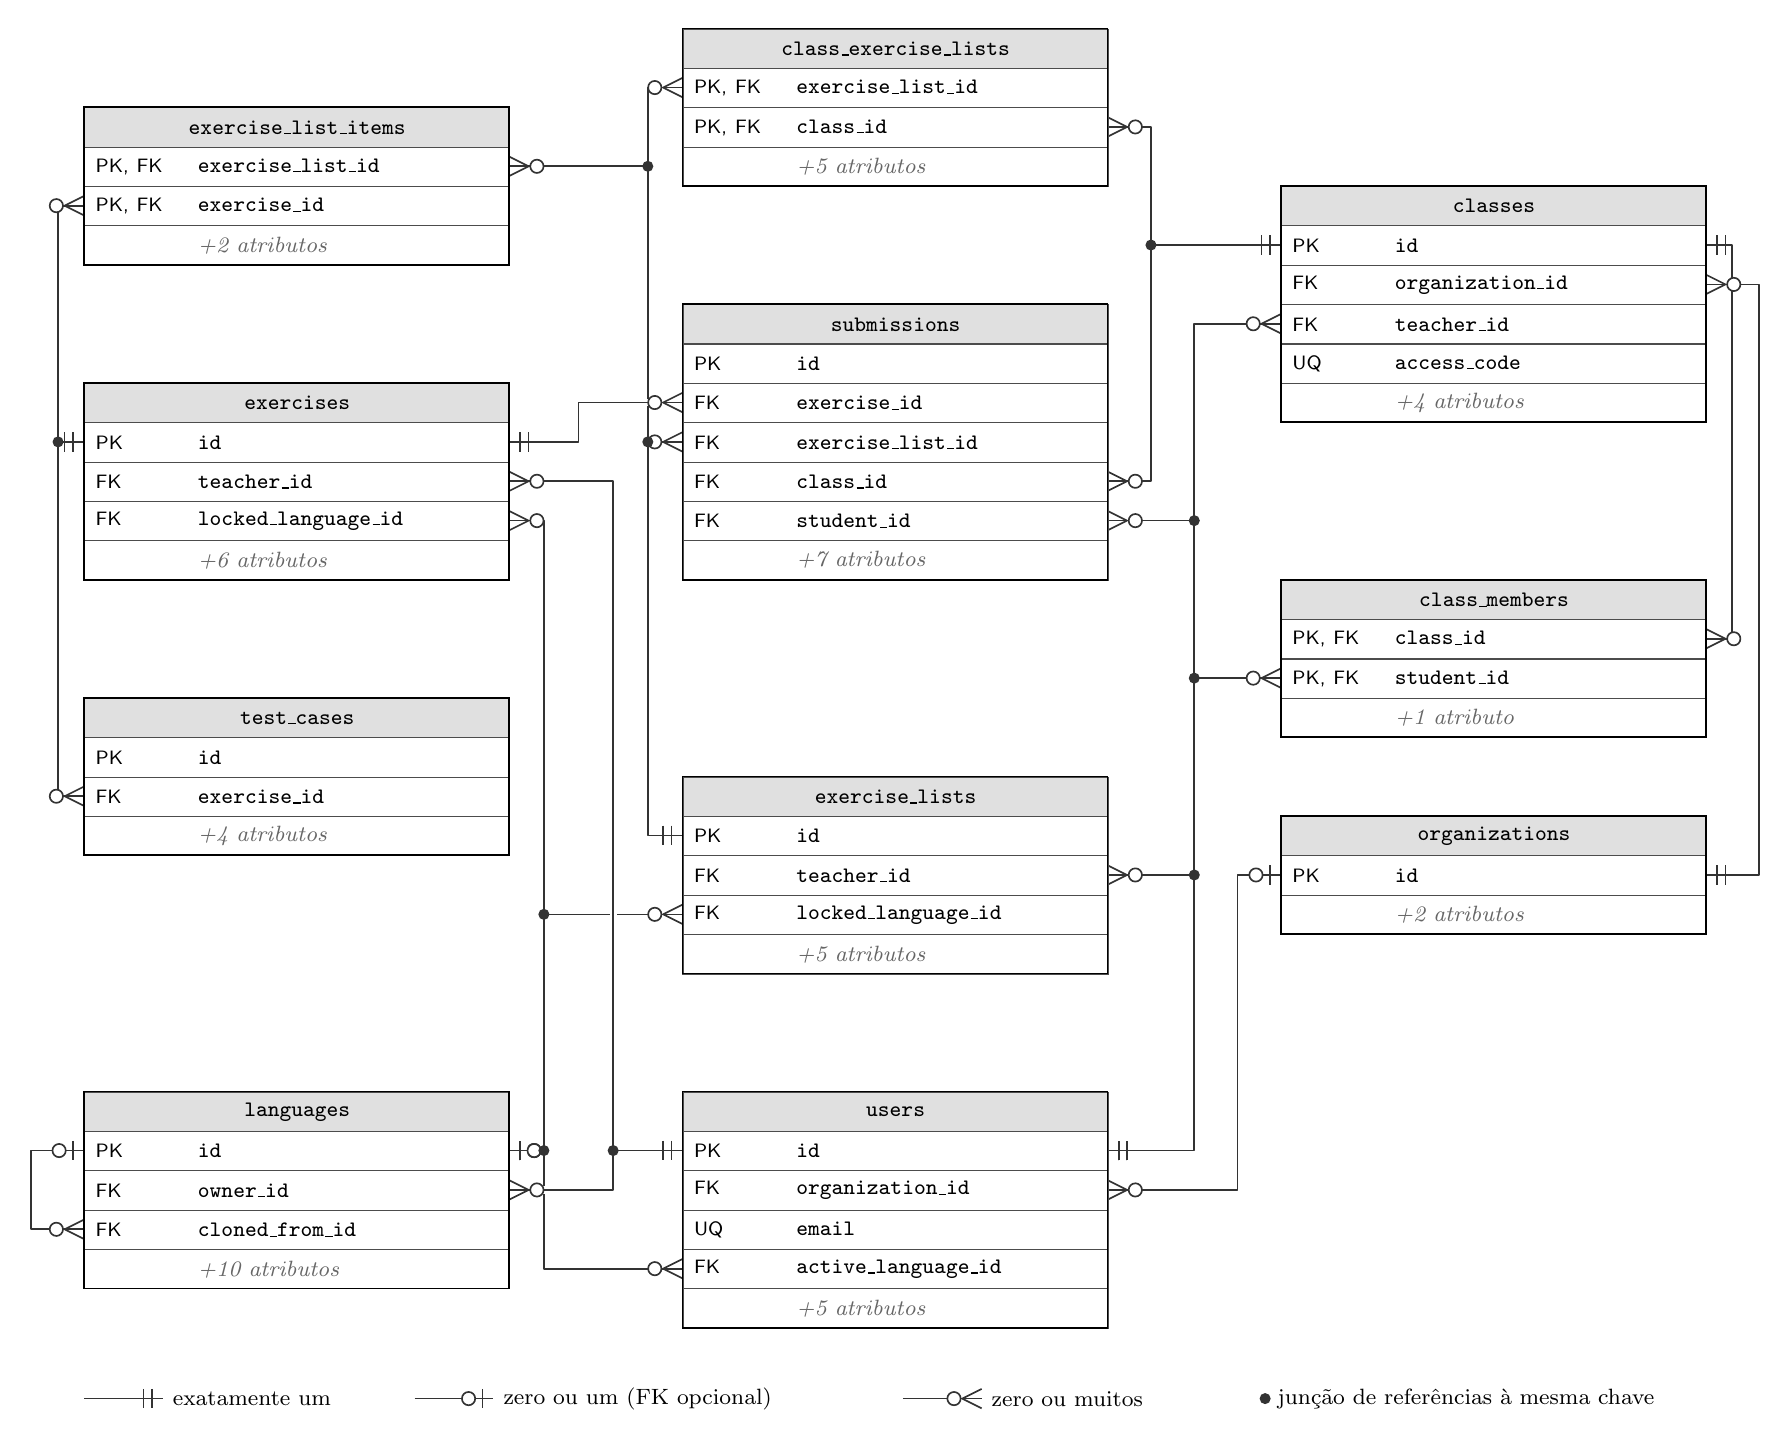
\begin{tikzpicture}[font=\footnotesize,cell/.style={draw=black!70,anchor=north west,minimum width=5.4cm,text width=5.12cm,minimum height=0.5cm,inner xsep=0.14cm,inner ysep=0pt,align=left,fill=white},head/.style={cell,fill=black!12,align=center},rel/.style={semithick,draw=black!80,line join=round,preaction={draw=white,line width=2.6pt,-}}]
\draw[rel,{CF many0}-{CF one}] (7.60,-0.75) -- (7.16,-0.75) -- (7.16,-10.25) -- (7.60,-10.25);
\draw[rel,{CF many0}-{CF one}] (5.40,-1.75) -- (7.16,-1.75) -- (7.16,-10.25) -- (7.60,-10.25);
\draw[rel,{CF many0}-{CF one}] (7.60,-5.25) -- (7.16,-5.25) -- (7.16,-10.25) -- (7.60,-10.25);
\fill[black!80] (7.16,-5.25) circle (2pt);
\fill[black!80] (7.16,-1.75) circle (2pt);
\draw[rel,{CF many0}-{CF one}] (13.00,-1.25) -- (13.55,-1.25) -- (13.55,-2.75) -- (15.20,-2.75);
\draw[rel,{CF many0}-{CF one}] (13.00,-5.75) -- (13.55,-5.75) -- (13.55,-2.75) -- (15.20,-2.75);
\fill[black!80] (13.55,-2.75) circle (2pt);
\draw[rel,{CF many0}-{CF one}] (20.60,-7.75) -- (20.93,-7.75) -- (20.93,-2.75) -- (20.60,-2.75);
\draw[rel,{CF many0}-{CF one}] (15.20,-8.25) -- (14.10,-8.25) -- (14.10,-14.25) -- (13.00,-14.25);
\draw[rel,{CF many0}-{CF one}] (15.20,-3.75) -- (14.10,-3.75) -- (14.10,-14.25) -- (13.00,-14.25);
\draw[rel,{CF many0}-{CF one}] (13.00,-10.75) -- (14.10,-10.75) -- (14.10,-14.25) -- (13.00,-14.25);
\draw[rel,{CF many0}-{CF one}] (13.00,-6.25) -- (14.10,-6.25) -- (14.10,-14.25) -- (13.00,-14.25);
\fill[black!80] (14.10,-10.75) circle (2pt);
\fill[black!80] (14.10,-8.25) circle (2pt);
\fill[black!80] (14.10,-6.25) circle (2pt);
\draw[rel,{CF many0}-{CF one}] (20.60,-3.25) -- (21.27,-3.25) -- (21.27,-10.75) -- (20.60,-10.75);
\draw[rel,{CF many0}-{CF one}] (0.00,-2.25) -- (-0.33,-2.25) -- (-0.33,-5.25) -- (0.00,-5.25);
\draw[rel,{CF many0}-{CF one}] (0.00,-9.75) -- (-0.33,-9.75) -- (-0.33,-5.25) -- (0.00,-5.25);
\fill[black!80] (-0.33,-5.25) circle (2pt);
\draw[rel,{CF many0}-{CF one0}] (7.60,-11.25) -- (5.84,-11.25) -- (5.84,-14.25) -- (5.40,-14.25);
\draw[rel,{CF many0}-{CF one0}] (5.40,-6.25) -- (5.84,-6.25) -- (5.84,-14.25) -- (5.40,-14.25);
\draw[rel,{CF many0}-{CF one0}] (7.60,-15.75) -- (5.84,-15.75) -- (5.84,-14.25) -- (5.40,-14.25);
\fill[black!80] (5.84,-14.25) circle (2pt);
\fill[black!80] (5.84,-11.25) circle (2pt);
\draw[rel,{CF many0}-{CF one}] (5.40,-5.75) -- (6.72,-5.75) -- (6.72,-14.25) -- (7.60,-14.25);
\draw[rel,{CF many0}-{CF one}] (5.40,-14.75) -- (6.72,-14.75) -- (6.72,-14.25) -- (7.60,-14.25);
\fill[black!80] (6.72,-14.25) circle (2pt);
\draw[rel,{CF many0}-{CF one0}] (0.00,-15.25) -- (-0.67,-15.25) -- (-0.67,-14.25) -- (0.00,-14.25);
\draw[rel,{CF many0}-{CF one}] (7.60,-4.75) -- (6.28,-4.75) -- (6.28,-5.25) -- (5.40,-5.25);
\draw[rel,{CF many0}-{CF one0}] (13.00,-14.75) -- (14.65,-14.75) -- (14.65,-10.75) -- (15.20,-10.75);
\node[head] at (7.60,0.00) {\texttt{class\_exercise\_lists}};
\node[cell] at (7.60,-0.50) {\makebox[1.3cm][l]{\textsf{\scriptsize PK, FK}}\texttt{exercise\_list\_id}};
\node[cell] at (7.60,-1.00) {\makebox[1.3cm][l]{\textsf{\scriptsize PK, FK}}\texttt{class\_id}};
\node[cell,text=black!60] at (7.60,-1.50) {\makebox[1.3cm][l]{}\textit{+5 atributos}};
\draw[semithick] (7.60,0.00) rectangle (13.00,-2.00);
\node[head] at (15.20,-7.00) {\texttt{class\_members}};
\node[cell] at (15.20,-7.50) {\makebox[1.3cm][l]{\textsf{\scriptsize PK, FK}}\texttt{class\_id}};
\node[cell] at (15.20,-8.00) {\makebox[1.3cm][l]{\textsf{\scriptsize PK, FK}}\texttt{student\_id}};
\node[cell,text=black!60] at (15.20,-8.50) {\makebox[1.3cm][l]{}\textit{+1 atributo}};
\draw[semithick] (15.20,-7.00) rectangle (20.60,-9.00);
\node[head] at (15.20,-2.00) {\texttt{classes}};
\node[cell] at (15.20,-2.50) {\makebox[1.3cm][l]{\textsf{\scriptsize PK}}\texttt{id}};
\node[cell] at (15.20,-3.00) {\makebox[1.3cm][l]{\textsf{\scriptsize FK}}\texttt{organization\_id}};
\node[cell] at (15.20,-3.50) {\makebox[1.3cm][l]{\textsf{\scriptsize FK}}\texttt{teacher\_id}};
\node[cell] at (15.20,-4.00) {\makebox[1.3cm][l]{\textsf{\scriptsize UQ}}\texttt{access\_code}};
\node[cell,text=black!60] at (15.20,-4.50) {\makebox[1.3cm][l]{}\textit{+4 atributos}};
\draw[semithick] (15.20,-2.00) rectangle (20.60,-5.00);
\node[head] at (0.00,-1.00) {\texttt{exercise\_list\_items}};
\node[cell] at (0.00,-1.50) {\makebox[1.3cm][l]{\textsf{\scriptsize PK, FK}}\texttt{exercise\_list\_id}};
\node[cell] at (0.00,-2.00) {\makebox[1.3cm][l]{\textsf{\scriptsize PK, FK}}\texttt{exercise\_id}};
\node[cell,text=black!60] at (0.00,-2.50) {\makebox[1.3cm][l]{}\textit{+2 atributos}};
\draw[semithick] (0.00,-1.00) rectangle (5.40,-3.00);
\node[head] at (7.60,-9.50) {\texttt{exercise\_lists}};
\node[cell] at (7.60,-10.00) {\makebox[1.3cm][l]{\textsf{\scriptsize PK}}\texttt{id}};
\node[cell] at (7.60,-10.50) {\makebox[1.3cm][l]{\textsf{\scriptsize FK}}\texttt{teacher\_id}};
\node[cell] at (7.60,-11.00) {\makebox[1.3cm][l]{\textsf{\scriptsize FK}}\texttt{locked\_language\_id}};
\node[cell,text=black!60] at (7.60,-11.50) {\makebox[1.3cm][l]{}\textit{+5 atributos}};
\draw[semithick] (7.60,-9.50) rectangle (13.00,-12.00);
\node[head] at (0.00,-4.50) {\texttt{exercises}};
\node[cell] at (0.00,-5.00) {\makebox[1.3cm][l]{\textsf{\scriptsize PK}}\texttt{id}};
\node[cell] at (0.00,-5.50) {\makebox[1.3cm][l]{\textsf{\scriptsize FK}}\texttt{teacher\_id}};
\node[cell] at (0.00,-6.00) {\makebox[1.3cm][l]{\textsf{\scriptsize FK}}\texttt{locked\_language\_id}};
\node[cell,text=black!60] at (0.00,-6.50) {\makebox[1.3cm][l]{}\textit{+6 atributos}};
\draw[semithick] (0.00,-4.50) rectangle (5.40,-7.00);
\node[head] at (0.00,-13.50) {\texttt{languages}};
\node[cell] at (0.00,-14.00) {\makebox[1.3cm][l]{\textsf{\scriptsize PK}}\texttt{id}};
\node[cell] at (0.00,-14.50) {\makebox[1.3cm][l]{\textsf{\scriptsize FK}}\texttt{owner\_id}};
\node[cell] at (0.00,-15.00) {\makebox[1.3cm][l]{\textsf{\scriptsize FK}}\texttt{cloned\_from\_id}};
\node[cell,text=black!60] at (0.00,-15.50) {\makebox[1.3cm][l]{}\textit{+10 atributos}};
\draw[semithick] (0.00,-13.50) rectangle (5.40,-16.00);
\node[head] at (15.20,-10.00) {\texttt{organizations}};
\node[cell] at (15.20,-10.50) {\makebox[1.3cm][l]{\textsf{\scriptsize PK}}\texttt{id}};
\node[cell,text=black!60] at (15.20,-11.00) {\makebox[1.3cm][l]{}\textit{+2 atributos}};
\draw[semithick] (15.20,-10.00) rectangle (20.60,-11.50);
\node[head] at (7.60,-3.50) {\texttt{submissions}};
\node[cell] at (7.60,-4.00) {\makebox[1.3cm][l]{\textsf{\scriptsize PK}}\texttt{id}};
\node[cell] at (7.60,-4.50) {\makebox[1.3cm][l]{\textsf{\scriptsize FK}}\texttt{exercise\_id}};
\node[cell] at (7.60,-5.00) {\makebox[1.3cm][l]{\textsf{\scriptsize FK}}\texttt{exercise\_list\_id}};
\node[cell] at (7.60,-5.50) {\makebox[1.3cm][l]{\textsf{\scriptsize FK}}\texttt{class\_id}};
\node[cell] at (7.60,-6.00) {\makebox[1.3cm][l]{\textsf{\scriptsize FK}}\texttt{student\_id}};
\node[cell,text=black!60] at (7.60,-6.50) {\makebox[1.3cm][l]{}\textit{+7 atributos}};
\draw[semithick] (7.60,-3.50) rectangle (13.00,-7.00);
\node[head] at (0.00,-8.50) {\texttt{test\_cases}};
\node[cell] at (0.00,-9.00) {\makebox[1.3cm][l]{\textsf{\scriptsize PK}}\texttt{id}};
\node[cell] at (0.00,-9.50) {\makebox[1.3cm][l]{\textsf{\scriptsize FK}}\texttt{exercise\_id}};
\node[cell,text=black!60] at (0.00,-10.00) {\makebox[1.3cm][l]{}\textit{+4 atributos}};
\draw[semithick] (0.00,-8.50) rectangle (5.40,-10.50);
\node[head] at (7.60,-13.50) {\texttt{users}};
\node[cell] at (7.60,-14.00) {\makebox[1.3cm][l]{\textsf{\scriptsize PK}}\texttt{id}};
\node[cell] at (7.60,-14.50) {\makebox[1.3cm][l]{\textsf{\scriptsize FK}}\texttt{organization\_id}};
\node[cell] at (7.60,-15.00) {\makebox[1.3cm][l]{\textsf{\scriptsize UQ}}\texttt{email}};
\node[cell] at (7.60,-15.50) {\makebox[1.3cm][l]{\textsf{\scriptsize FK}}\texttt{active\_language\_id}};
\node[cell,text=black!60] at (7.60,-16.00) {\makebox[1.3cm][l]{}\textit{+5 atributos}};
\draw[semithick] (7.60,-13.50) rectangle (13.00,-16.50);
\draw[rel,-{CF one}] (0,-17.40) -- ++(1,0) node[right,black] {exatamente um};
\draw[rel,-{CF one0}] (4.2,-17.40) -- ++(1,0) node[right,black] {zero ou um (FK opcional)};
\draw[rel,-{CF many0}] (10.4,-17.40) -- ++(1,0) node[right,black] {zero ou muitos};
\fill[black!80] (15.0,-17.40) circle (2pt) node[right,black,xshift=1pt] {junção de referências à mesma chave};
\end{tikzpicture}}

    \legend{Fonte: elaborado pelo autor a partir dos modelos SQLAlchemy do \textit{back-end}.}
\end{figure}
\FloatBarrier

Os dados de acesso e dos alunos ficam nas tabelas \texttt{organizations}, \texttt{users}, \texttt{classes} e \texttt{class\_members}. Todos os usuários estão na mesma tabela e se distinguem pelo campo \texttt{role}, cujos valores são \texttt{ADMIN}, \texttt{TEACHER}, \texttt{STUDENT}, \texttt{COMMUNITY} e \texttt{SYSTEM}; a correspondência desses papéis com os atores do diagrama de casos de uso foi apresentada na Seção~\ref{sec:casos-de-uso}. A tabela de usuários guarda ainda nome, e-mail, o resumo criptográfico da senha, foto e biografia, e o vínculo com uma organização é opcional. A turma referencia uma organização e o professor responsável e tem um código de acesso único, que o aluno informa para ingressar nela. O ingresso é registrado em \texttt{class\_members}, cuja chave primária combina turma e aluno.

As personalizações ficam na tabela \texttt{languages}. Cada linguagem tem um proprietário, nome, descrição e a configuração completa em um campo JSON, com as palavras-chave, os operadores, os literais booleanos, os delimitadores, o terminador de instrução e os modos escolhidos no assistente. A tabela registra também se a linguagem foi publicada no catálogo da comunidade e, quando ela foi importada de outra, a linguagem de origem, no campo \texttt{cloned\_from\_id}. O campo \texttt{active\_language\_id} da tabela de usuários aponta para a linguagem ativa de cada usuário autenticado. Um mesmo usuário não pode ter duas linguagens com o mesmo nome. A customização em uso no editor e os arquivos do sistema de arquivos virtual ficam no armazenamento local do navegador, e por isso o visitante consegue usar a personalização sem conta.

As atividades são distribuídas entre \texttt{exercises}, \texttt{test\_cases}, \texttt{exercise\_lists} e \texttt{exercise\_list\_items}. Exercícios e listas pertencem a um professor e têm uma política de linguagem, aberta (\texttt{OPEN}) ou travada (\texttt{LOCKED}); uma restrição de verificação exige que a linguagem obrigatória, \texttt{locked\_language\_id}, esteja preenchida exatamente quando a política é \texttt{LOCKED}. Os casos de teste pertencem a um exercício e guardam a entrada e a saída esperada. Os itens de lista associam exercícios a listas, com peso na nota e ordem de apresentação.

A publicação de uma lista para uma turma é registrada em \texttt{class\_exercise\_lists}, com prazo, nota total e quantidade mínima de exercícios. A tabela \texttt{submissions} registra cada tentativa do aluno: referencia o exercício, a lista, a turma e o estudante e guarda uma cópia do código e da configuração da linguagem no momento do envio, nos campos \texttt{code\_snapshot} e \texttt{language\_snapshot}. Essas cópias preservam o contexto da tentativa mesmo que o aluno altere depois o código ou a linguagem. A submissão guarda também o estado, a pontuação, o comentário do professor, a data de envio e o resultado de cada caso de teste, em uma lista JSON. O dicionário de dados completo, com todos os atributos, está no texto complementar de Victor de Souza Vilela da Silva.
